\section{Mathematical description}

The physical model can be described by ordinary differential equations (ODEs), subdividing the system into single components: DC motor, gear, first spring, first mass, second spring, second mass. The parameters used are the nominal values defined in the manuals of components setup. This formulation of the problem can be useful in the following chapters, when the controller design will depend on the state-space realization or on the transfer functions.
\begin{figure*}[h]
	\centering
	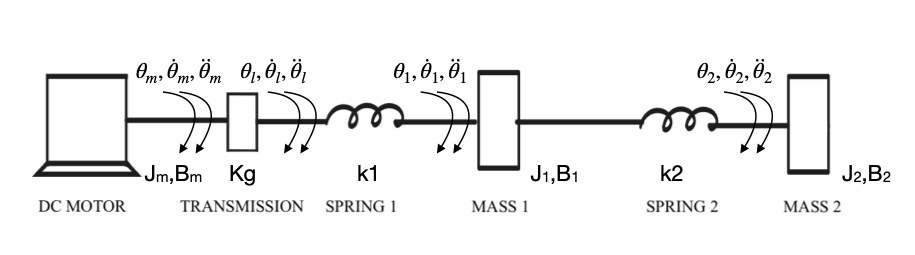
\includegraphics[width=0.8\columnwidth]{system_scheme}
	\caption{Scheme of the physical model}
\end{figure*}

% Equazioni componenti
\textit{Model of the motor and gear box}
\begin{subequations}
	\begin{align}
		V &= R_m i + L_m \frac{d}{dt}i + k_m \dot{\theta}_m \\
		\tau_m &= \eta_m k_t i \\
		\tau_{ml} &= \eta_g K_g \tau_m = \eta_m \eta_g K_g k_t i\\
		&= -J_m \ddot{\theta}_l - B_m \dot{\theta}_l - K_{s1} ( \theta_l - \theta_1 ) \qquad  \theta_l = \frac {1}{K_g} \theta_m \\
		\label{fig:model_equations}
	\end{align}
\end{subequations}

\textit{Model of the \acrshort{1-dof} system}
\begin{equation}
	J_1 \ddot{\theta}_1 + B_1 \dot{\theta}_1 = K_{s_1} ( \theta_l - \theta_1 )
\end{equation}

\textit{Model of the \acrshort{2-dof} system}
\begin{subequations}
	\begin{align}
		J_1 \ddot{\theta}_1 + B_1 \dot{\theta}_1 &= K_{s_1} ( \theta_l - \theta_1 ) - K_{s_2} ( \theta_1 - \theta_2 ) \\
		J_2 \ddot{\theta}_2 + B_2 \dot{\theta}_2 &= K_{s_2} ( \theta_1 - \theta_2 )
	\end{align}
\end{subequations}

% Forma di stato
\textit{State-space representation of the complete 1 d.o.f. system}
\begin{equation}
	\begin{bmatrix}
		\dot{i} \\
		\dot{\theta}_l \\
		\ddot{\theta}_l \\
		\dot{\theta}_1 \\
		\ddot{\theta}_1
	\end{bmatrix}
	=
	\begin{bmatrix}
		-\frac{R_m}{L_m} & 0 & -\frac{k_m K_g}{L_m} & 0 & 0 \\
		0 & 0 &1 & 0 & 0 \\
		\frac{\eta_m \eta_g k_t K_g}{J_m} & -\frac{K_{s_1}}{J_m} & -\frac{B_m}{J_m} & \frac{K_{s_1}}{J_m} & 0 \\
		0 & 0 & 0 & 0 & 1 \\
		0 & \frac{K_{s_1}}{J_1} & 0 & -\frac{K_{s_1}}{J_1} & -\frac{B_1}{J_1}
	\end{bmatrix}
	\begin{bmatrix}
		i \\
		\theta_l \\
		\dot{\theta}_l \\
		\theta_1 \\
		\dot{\theta}_1
	\end{bmatrix}
	+
	\begin{bmatrix}
		\frac{1}{L_m} \\
		0 \\
		0 \\
		0 \\
		0
	\end{bmatrix}
	V
\end{equation}

\textit{State-space representation of the complete 2 d.o.f. system}
\begin{equation}
	\begin{bmatrix}
		\dot{i} \\
		\dot{\theta}_l \\
		\ddot{\theta}_l \\
		\dot{\theta}_1 \\
		\ddot{\theta}_1 \\
		\dot{\theta}_2 \\
		\ddot{\theta}_2
	\end{bmatrix}
	=
	\begin{bmatrix}
		-\frac{R_m}{L_m} & 0 & -\frac{k_m K_g}{L_m} & 0 & 0 & 0 & 0 \\
		0 & 0 &1 & 0 & 0 & 0 & 0 \\
		\frac{\eta_m \eta_g k_t K_g}{J_m} & -\frac{K_{s_1}}{J_m} & -\frac{B_m}{J_m} & \frac{K_{s_1}}{J_m} & 0 & 0 & 0 \\
		0 & 0 & 0 & 0 & 1 & 0 & 0 \\
		0 & \frac{K_{s_1}}{J_1} & 0 & -\frac{K_{s_1}+K_{s_2}}{J_1} & -\frac{B_1}{J_1} & \frac{K_{s_2}}{J_1} & 0 \\
		0 & 0 & 0 & 0 & 0 & 0 & 1 \\
		0 & 0 & 0 & \frac{K_{s_2}}{J_2} & 0 & -\frac{K_{s_2}}{J_2} & -\frac{B_2}{J_2}
	\end{bmatrix}
	\begin{bmatrix}
		i \\
		\theta_l \\
		\dot{\theta}_l \\
		\theta_1 \\
		\dot{\theta}_1 \\
		\theta_2 \\
		\dot{\theta}_2
	\end{bmatrix}
	+
	\begin{bmatrix}
		\frac{1}{L_m} \\
		0 \\
		0 \\
		0 \\
		0 \\
		0 \\
		0
	\end{bmatrix}
	V
\end{equation}

From this mathematical formulation, it is easy to check (thanks to MATLAB functions  \textit{ctrb} e \textit{obsv}) the controllability by means of the voltage applied to the motor and the system observability.
The system having just one rotating mass is controllable only in two state variables over five: surely, one of those is the current (directly affected by the input), the other is one among the remaining. On the other hand, the observability matrix~$M_O$ is full rank; however, it must be considered that the current~$i$ dynamics is extremely rapid (the time constant is defined as~$\tau_i = \frac{L_m}{R_m} = 7.56\ 10^{-5} \ s$), then the sampling time~($T_s = 2 ms$) prevents its observation even with a current sensor installed on the motor.
Similarly to this case, it can be expected that also the 2-d.o.f. system is not fully controllable. \\

Since the current dynamics cannot be verified by experimental data, we have decided to ignore it~(the rest of the model is not significantly affected by that, since its transient is definitely negligible): in the following model, the current statically depends on the input voltage and the electromotive force (back-emf).\\
% Forma di stato ridotta
\textit{State-space representation of the reduced 1-d.o.f. system}
\begin{equation}
	\begin{bmatrix}
		\dot{\theta}_l \\
		\ddot{\theta}_l \\
		\dot{\theta}_1 \\
		\ddot{\theta}_1
	\end{bmatrix}
	=
	\begin{bmatrix}
		0 &1 & 0 & 0 \\
		-\frac{K_{s_1}}{J_m} & -\frac{B_m}{J_m}-\frac{\eta_m \eta_g k_t k_m {K_g}^2}{R_m J_m}  & \frac{K_{s_1}}{J_m} & 0 \\
		0 & 0 & 0 & 1 \\
		\frac{K_{s_1}}{J_1} & 0 & -\frac{K_{s_1}}{J_1} & -\frac{B_1}{J_1}
	\end{bmatrix}
	\begin{bmatrix}
		\theta_l \\
		\dot{\theta}_l \\
		\theta_1 \\
		\dot{\theta}_1
	\end{bmatrix}
	+
	\begin{bmatrix}
		0 \\
		\frac{\eta_m \eta_g k_t K_g}{R_m J_m} \\
		0 \\
		0
	\end{bmatrix}
	V
\end{equation}

\textit{State-space representation of the reduced 2-d.o.f. system}
\begin{equation}
	\begin{bmatrix}
		\dot{\theta}_l \\
		\ddot{\theta}_l \\
		\dot{\theta}_1 \\
		\ddot{\theta}_1 \\
		\dot{\theta}_2 \\
		\ddot{\theta}_2
	\end{bmatrix}
	=
	\begin{bmatrix}
		0 &1 & 0 & 0 & 0 & 0 \\
		-\frac{K_{s_1}}{J_m} & -\frac{B_m}{J_m}-\frac{\eta_m \eta_g k_t k_m {K_g}^2}{R_m J_m}  & \frac{K_{s_1}}{J_m} & 0 & 0 & 0 \\
		0 & 0 & 0 & 1 & 0 & 0 \\
		\frac{K_{s_1}}{J_1} & 0 & -\frac{K_{s_1}+K_{s_2}}{J_1} & -\frac{B_1}{J_1} & \frac{K_{s_2}}{J_1} & 0 \\
		0 & 0 & 0 & 0 & 0 & 1 \\
		0 & 0 & \frac{K_{s_2}}{J_2} & 0 & -\frac{K_{s_2}}{J_2} & -\frac{B_2}{J_2}
	\end{bmatrix}
	\begin{bmatrix}
		\theta_l \\
		\dot{\theta}_1 \\
		\theta_1 \\
		\dot{\theta}_1 \\
		\theta_2 \\
		\dot{\theta}_2
	\end{bmatrix}
	+
	\begin{bmatrix}
		0 \\
		\frac{\eta_m \eta_g k_t K_g}{R_m J_m} \\
		0 \\
		0 \\
		0 \\
		0
	\end{bmatrix}
	V
\end{equation}
This time, checking again the controllability and observability of the reduced order system, matrices~$M_R$ e $M_O$ are full rank. \\

In order to validate this model, some experiments on the real system have been performed. Firstly, only one mass, then, two masses in cascade were linked to the shaft. By imposing to the motor a certain voltage, the open-loop response has been compared to the Simulink simulation (based on the model previously illustrated).

\paragraph{Experiments input}
The experiments, aimed at identifying and validating the model, have been performed by imposing a voltage to the motor. They can be classified in two types: steps (multiple in time and of different size) and variable frequency sine waves. The range of applied voltages~($\pm 10\ V$) is constrained by the motor physical limitations.

At first, the static gain of the transfer function between the control input of the motor and the first mass speed~($G_{V,\dot{\theta}_1}$) has been checked. To do so, a constant voltage has been imposed; once the transient of first mass settlement is over, it is clear that the mathematical model underestimates the steady-state speed.
The first approach has been that of changing the model parameters whose effect on the static gain is more significant: the rotor resistance~($R_m$), the motor efficiency~($\eta_m$), the mechanical efficiency of the gear~($\eta_g$), the current-torque constant~($k_t$) and the mass speed-voltage constant (~$k_m$, responsible of the back-emf).

Thanks to the experiments, it has been noticed that the real system behavior is not exactely linear with respect to the imposed voltage. Some physical interpretations have been proposed: the mechanical efficiency of the motor~($\eta_g$) is probably underestimated at low speeds; then, the~$k_m$ constant (that generates the back-emf), is very difficult to be estimated, since its effect on the motor power is quite significant at high speed, but almost negligible at low speed.

% parametri modificati ---> G_opt

The variable frequency sine wave experiments suggest another significant difference between the physical model and the nominal one. Here, it is visible that resonance frequency of the nominal model is greater that the real one; anyway, the amplitude of the oscillations at those frequencies is comparable. \\
This fact affects also the step response transient: the initial overshoot and later oscillations depend on complex conjugate poles, linked to the physical parameters of springs and masses (spring stiffness~$K_s$, mass inertia~$J$, mass friction coefficient~$B$). \\

A tuning of the static gain does not allow an improvement of the mathematical model in the transient behavior. However, manually changing all the other parameters would be particularly difficult, since it is a trial-and-error approach based on no precise rational reasoning (it must be considered also, indeed, that nominal parameters shown in the reference manual are obtained experimentally).
A solution to this problem is to untie our approach from the purely mathematical model (i.e. white-box) and use experimental data.

\section{Black-box identification}

\textit{Black-box identification with a parametric method of TF in time-domain} \\

\par A black-box approach totally loses a connection to the mathematical model and its physical dimensions; on the contrary, it is exclusively based on data collected by experiments in laboratory.
For this reason, it is reasonable to estimate only the transfer function of our interest (according to the design of the controller of speed, designed later):~$G_{V,\dot{\theta}_1}$ or~$G_{V,\dot{\theta}_2}$, meaning the transfer functions from the voltage (input) and the masses speed. \\

Masses speeds (generated by the derivation of encoder data) are collected in a set of experiments by using the Matlab functions~\textit{iddata()} e~\textit{merge()}. So, the obtained data are the input of the~\textit{tfest()} function: the obtained output is the identified black-box model. \\

Keeping in mind that the transfer function only sees observable and controllable poles, a first method to impose the number of poles in the identification function is looking at the computer results: if the obtained transfer function does not change by adding more poles, then the order of the system has been obtained.
By this procedure, it has been found a~$3^{rd}$ order transfer function, with 2 positive-real part zeros: in this way, the phase loss at high frequency of the nominal and empirical models coincide. On the other hand, the gain at that frequency is much less inclined.

\begin{figure*}[h]
	\centering
	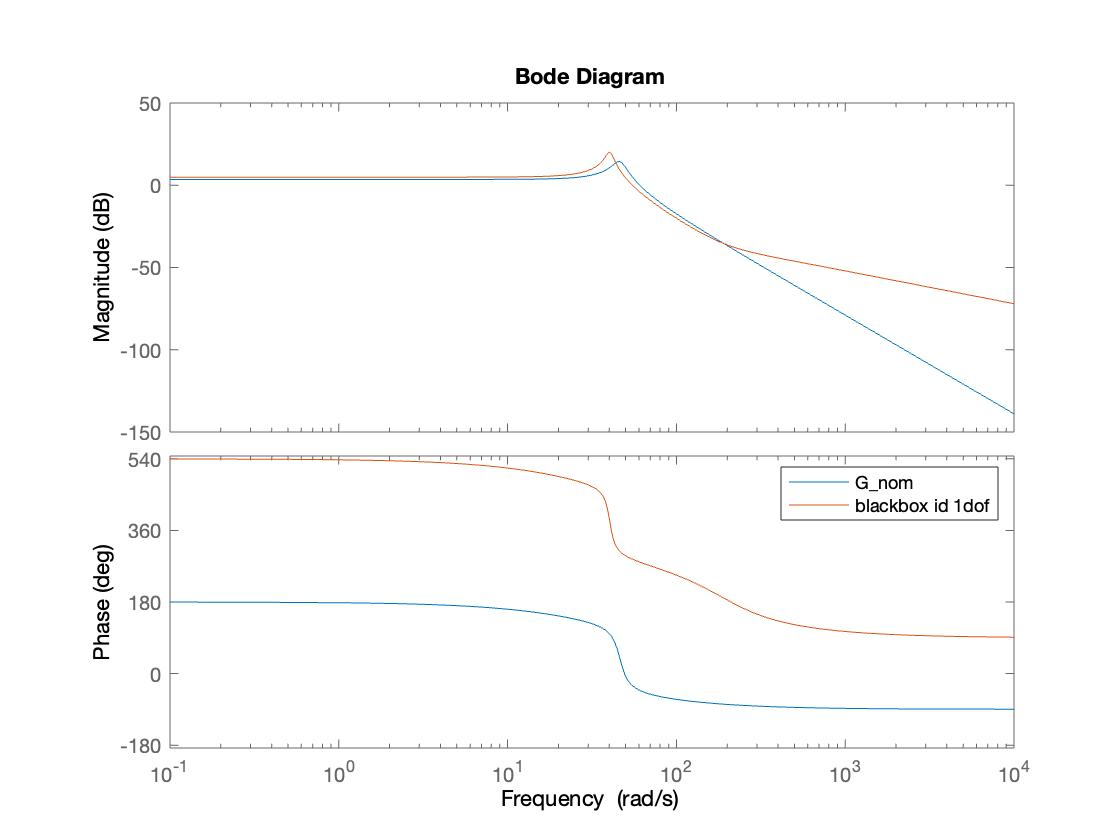
\includegraphics[width=\columnwidth]{black_1dof_withZeros}
	\caption{1-dof system. Transfer functions comparison, with zeros in blackbox}
\end{figure*}
\begin{figure*}[h]
	\centering
	\begin{subfigure}{\columnwidth}
%		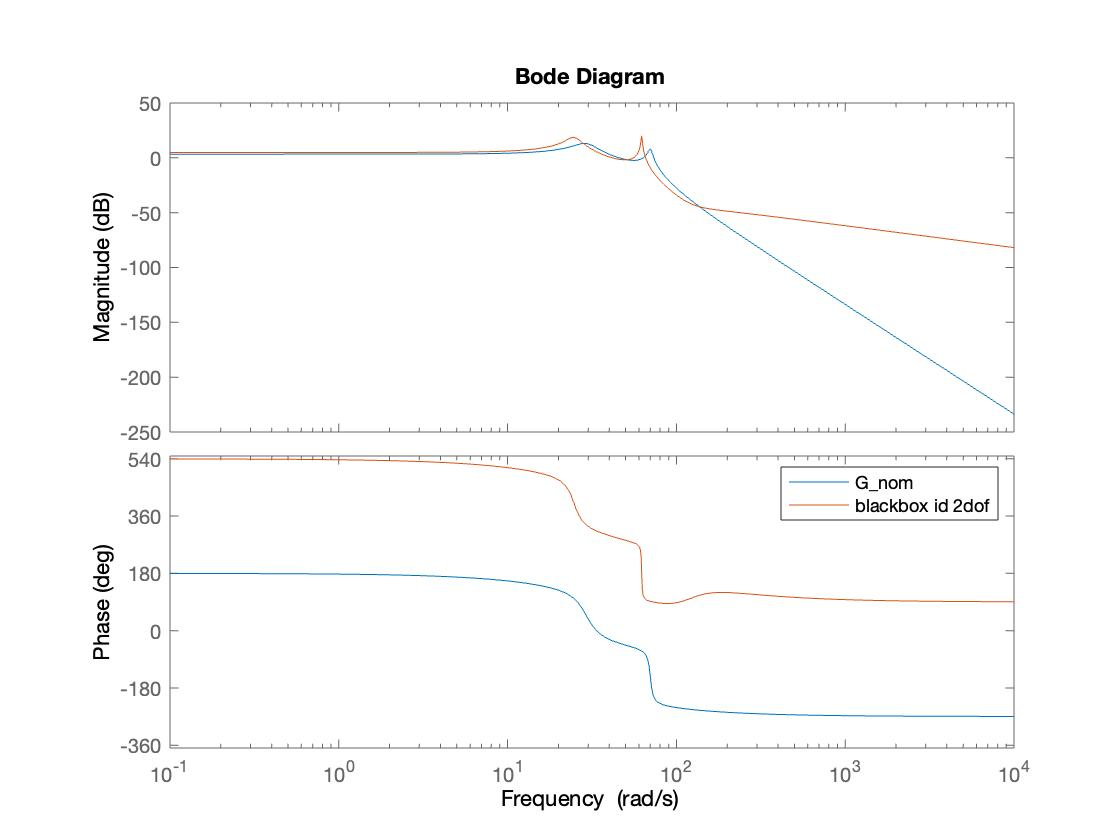
\includegraphics[width=\columnwidth]{black_2dof_withZeros}
	\end{subfigure}
	\begin{subfigure}{\columnwidth}
		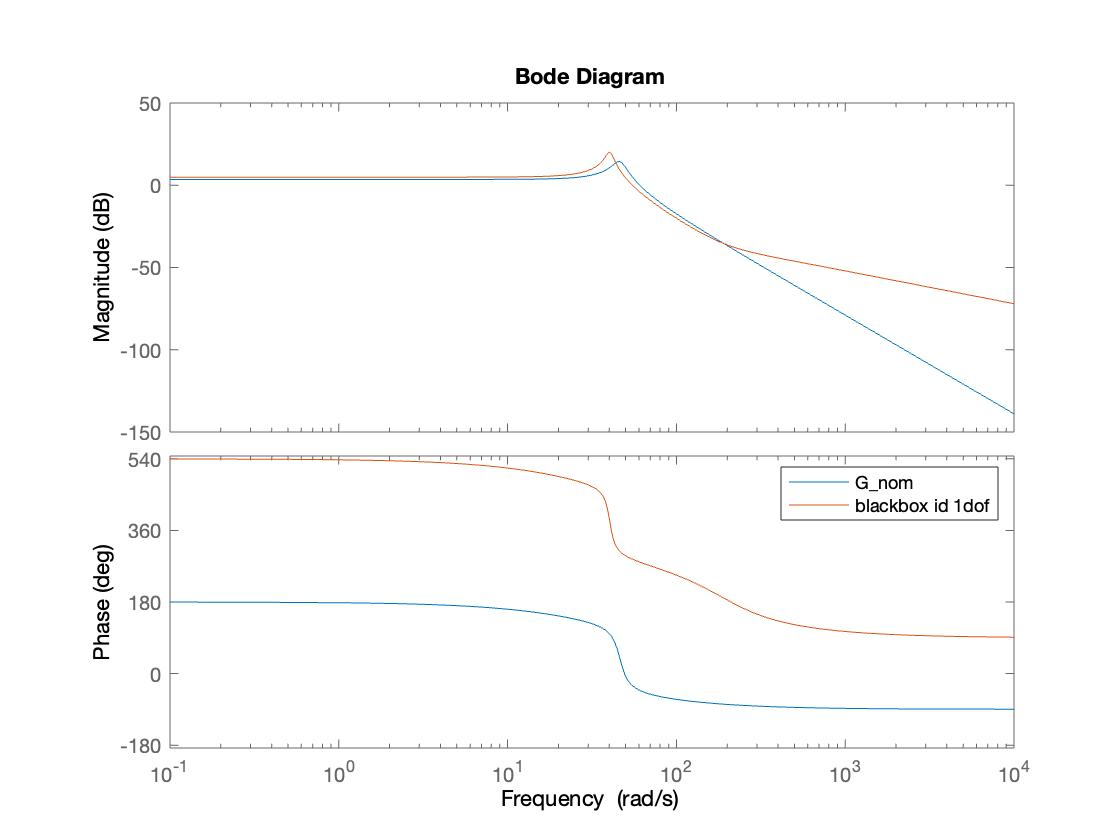
\includegraphics[width=\columnwidth]{black_1dof_withZeros}
	\end{subfigure}
	\caption{2-dof system. Transfer functions comparison, with zeros in blackbox}
\end{figure*}

To overcome this problem, it has been decided to impose the number of both poles and zeros, to be equal to the transfer function structure computed from the white-box model. Therefore, the 1 dof system has 3 poles and 0 zeros, while the 2 dof system has 5 poles and 0 zeros.
In addition to the physical model poles, it must be considered the low-pass filter for the speed measurement noise. \\
In this way, both module and phase Bode diagrams are very similar to the mathematical ones at every frequency.

\begin{figure*}[h]
	\centering
	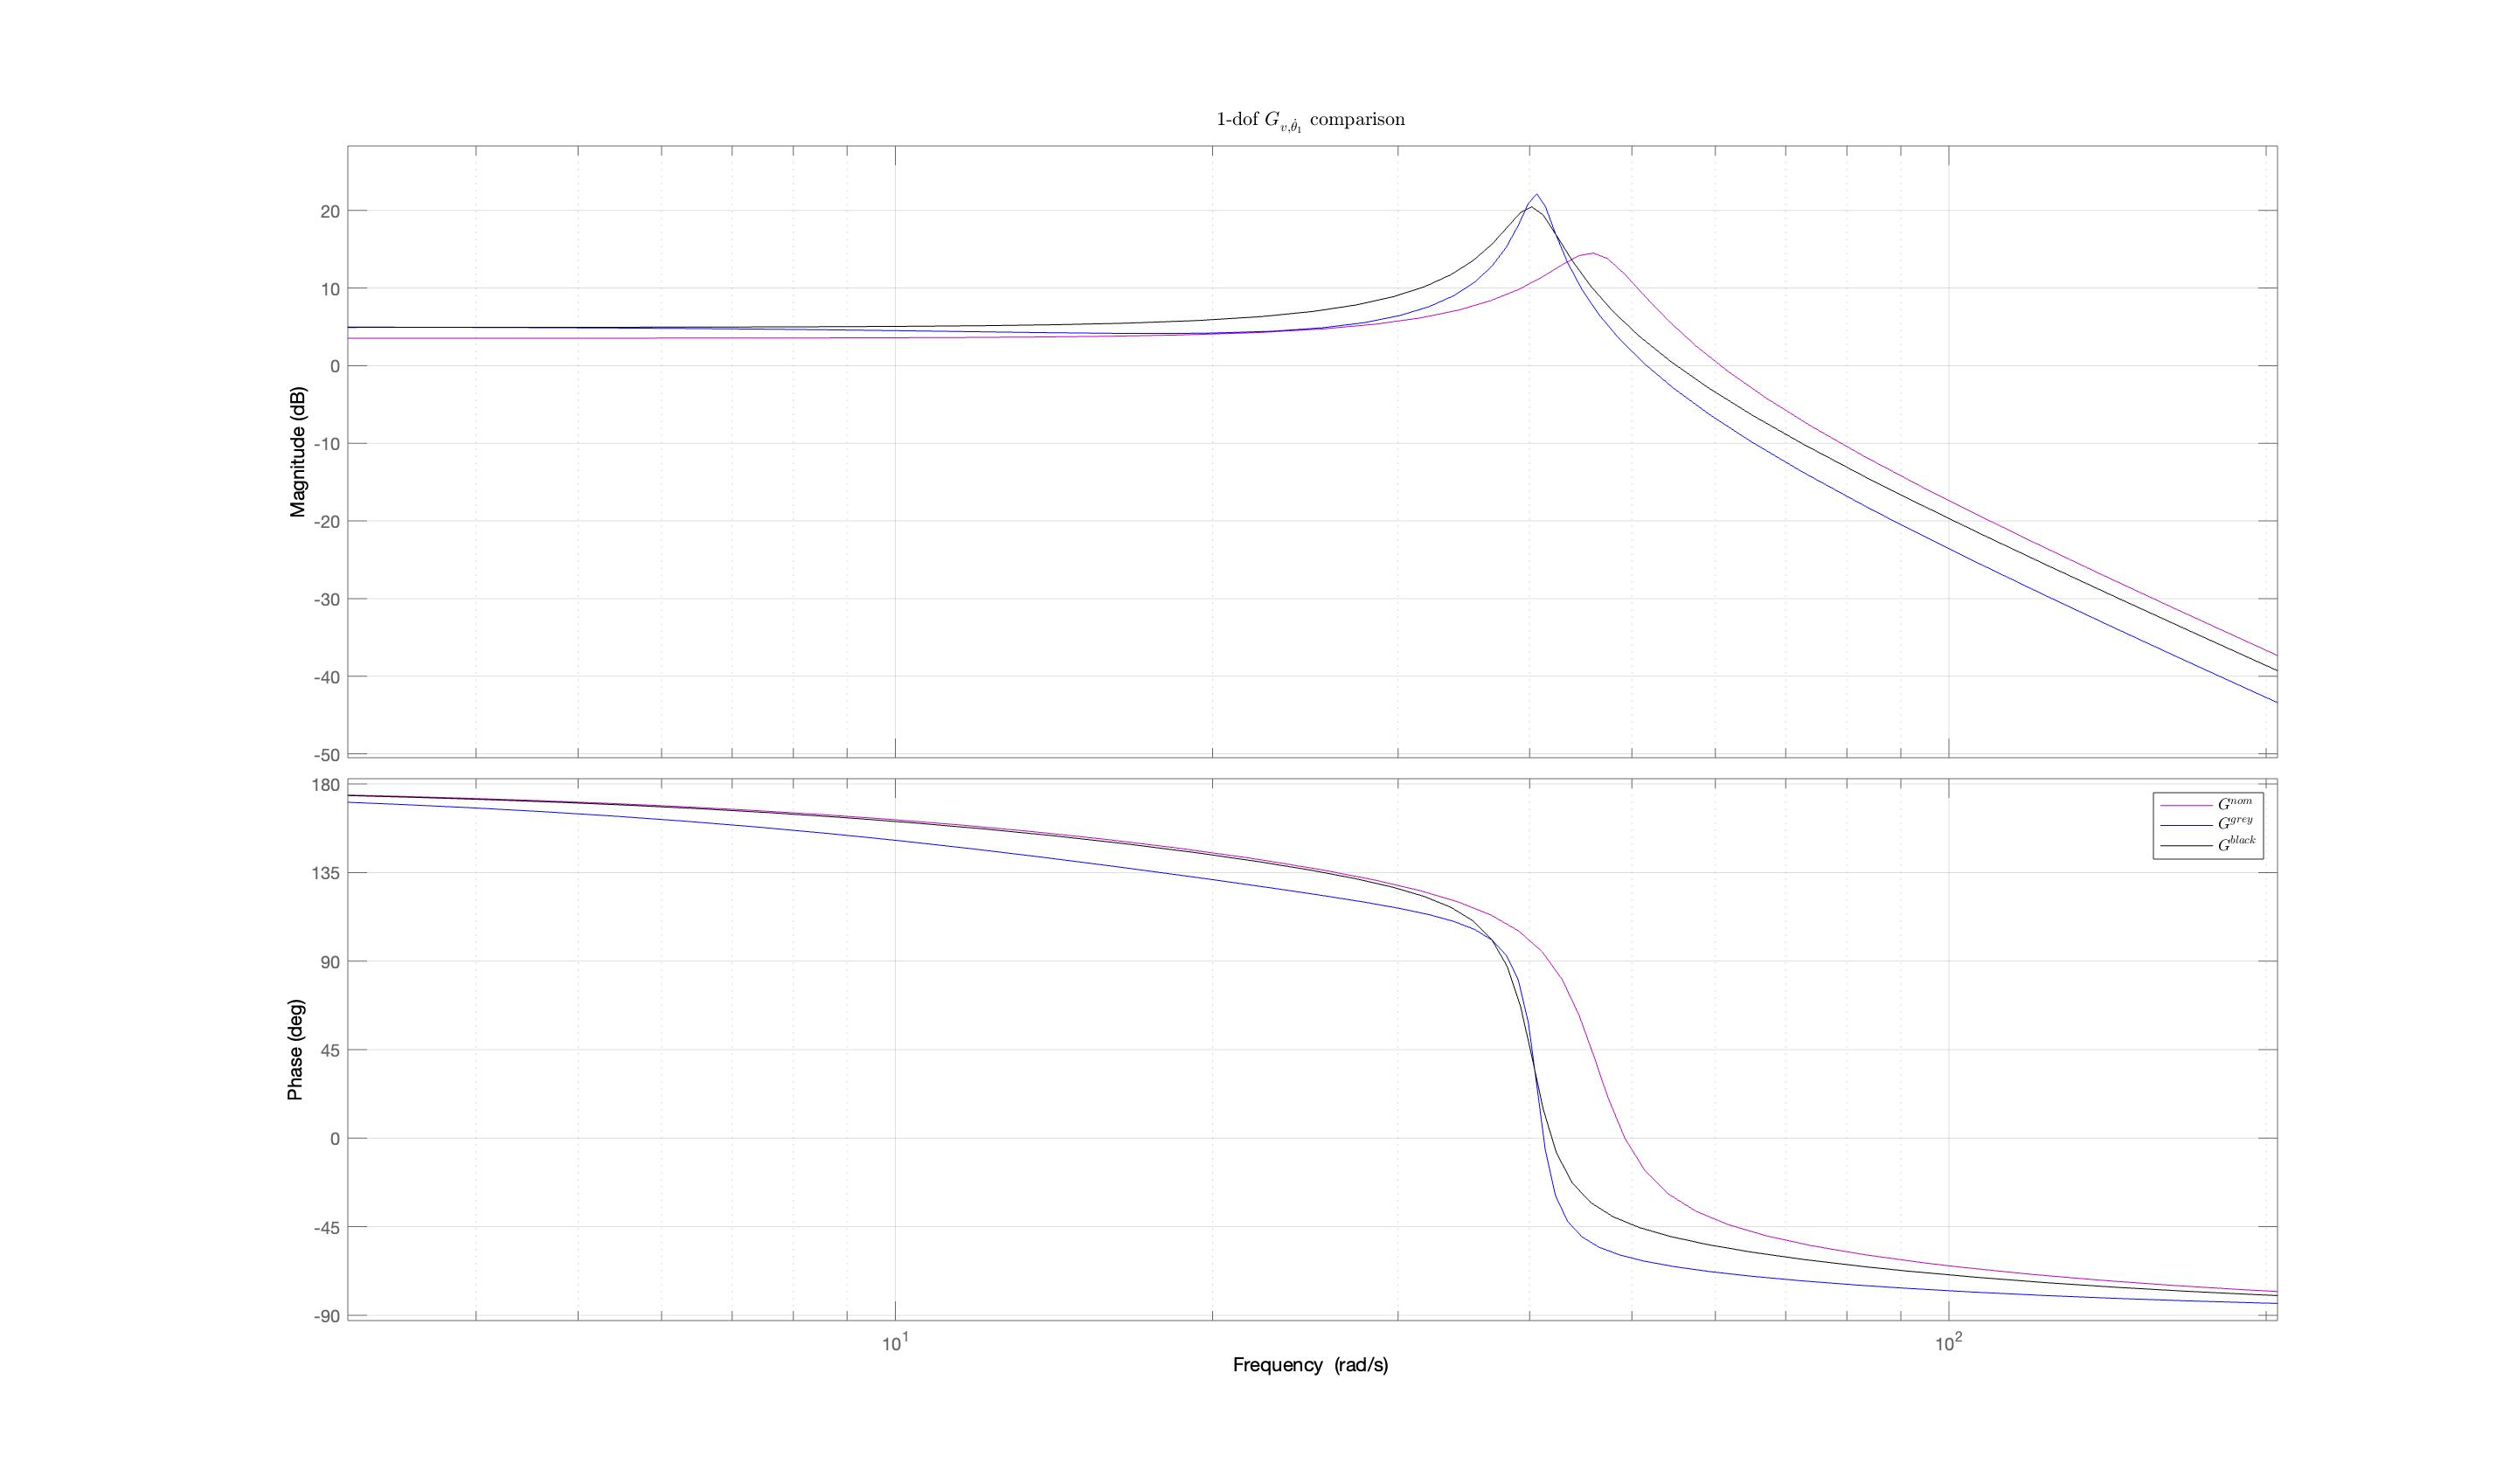
\includegraphics[width=\columnwidth]{1dof_g_v_w1}
	\caption{1-dof system. Transfer functions comparison, no zeros in blackbox}
\end{figure*}

\begin{figure*}[h]
	\centering
	\begin{subfigure}{0.45\columnwidth}
		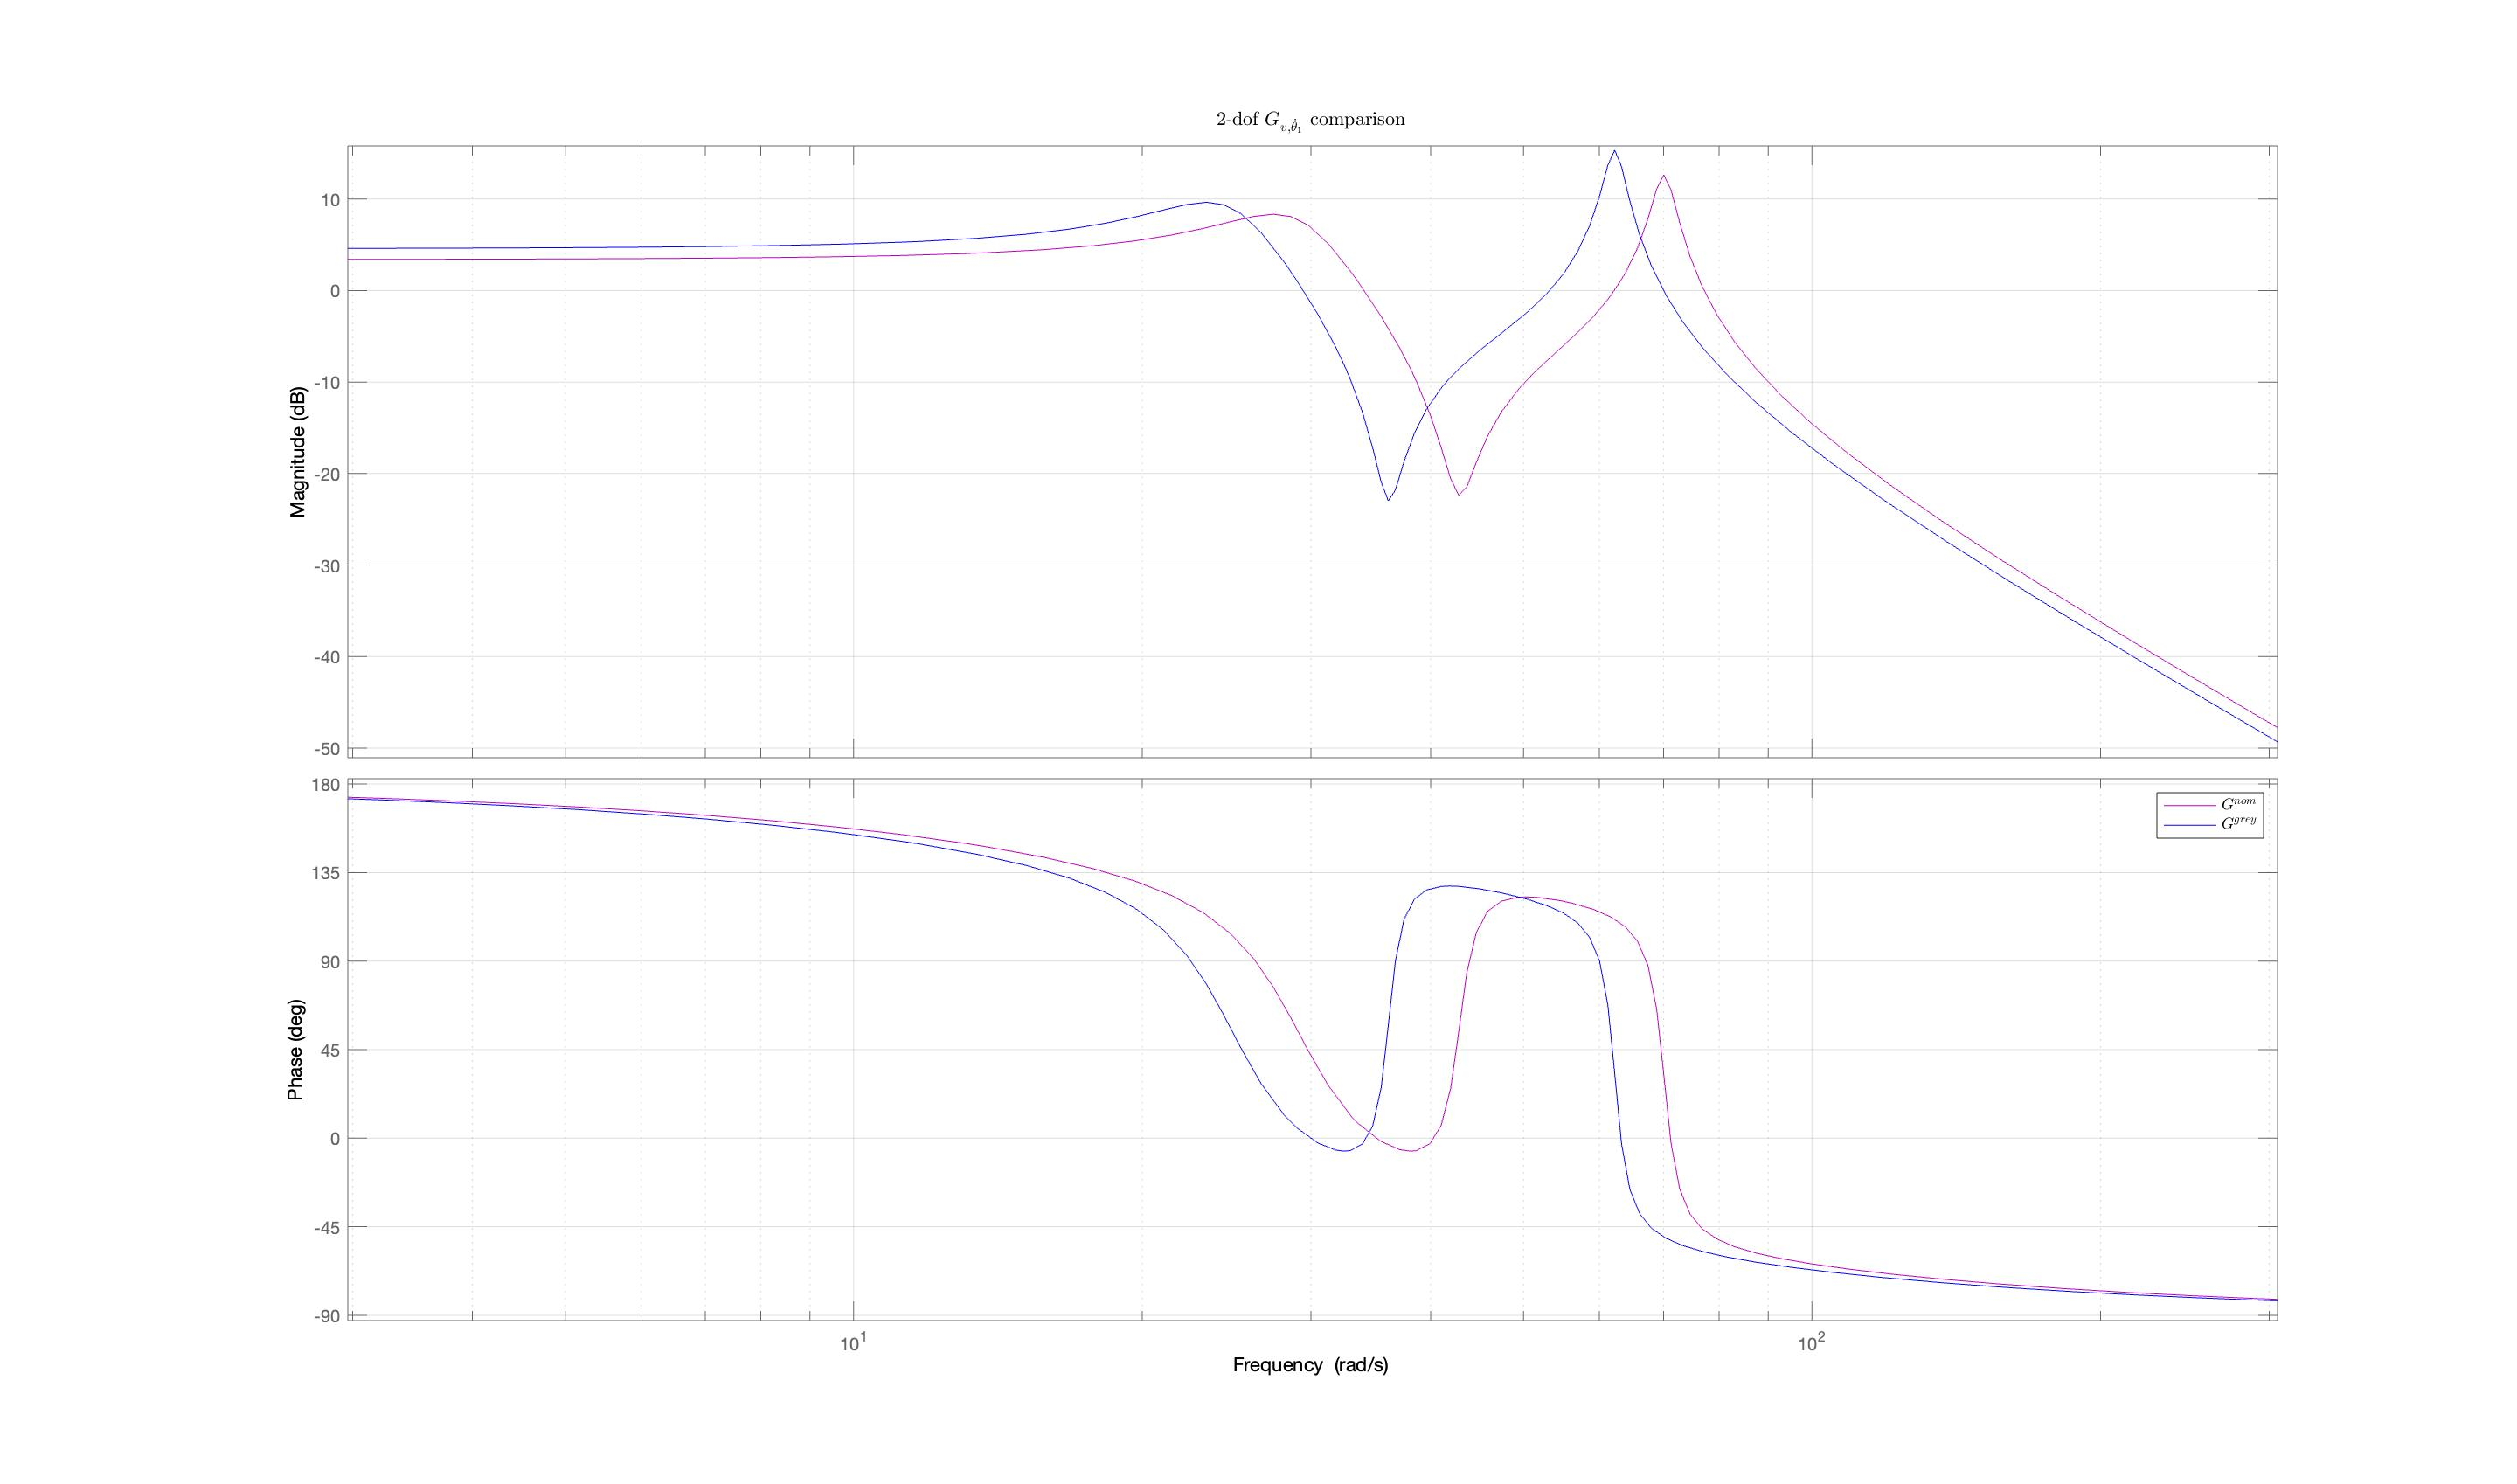
\includegraphics[width=\textwidth]{2dof_g_v_w1}
	\end{subfigure}
	\begin{subfigure}{0.45\columnwidth}
		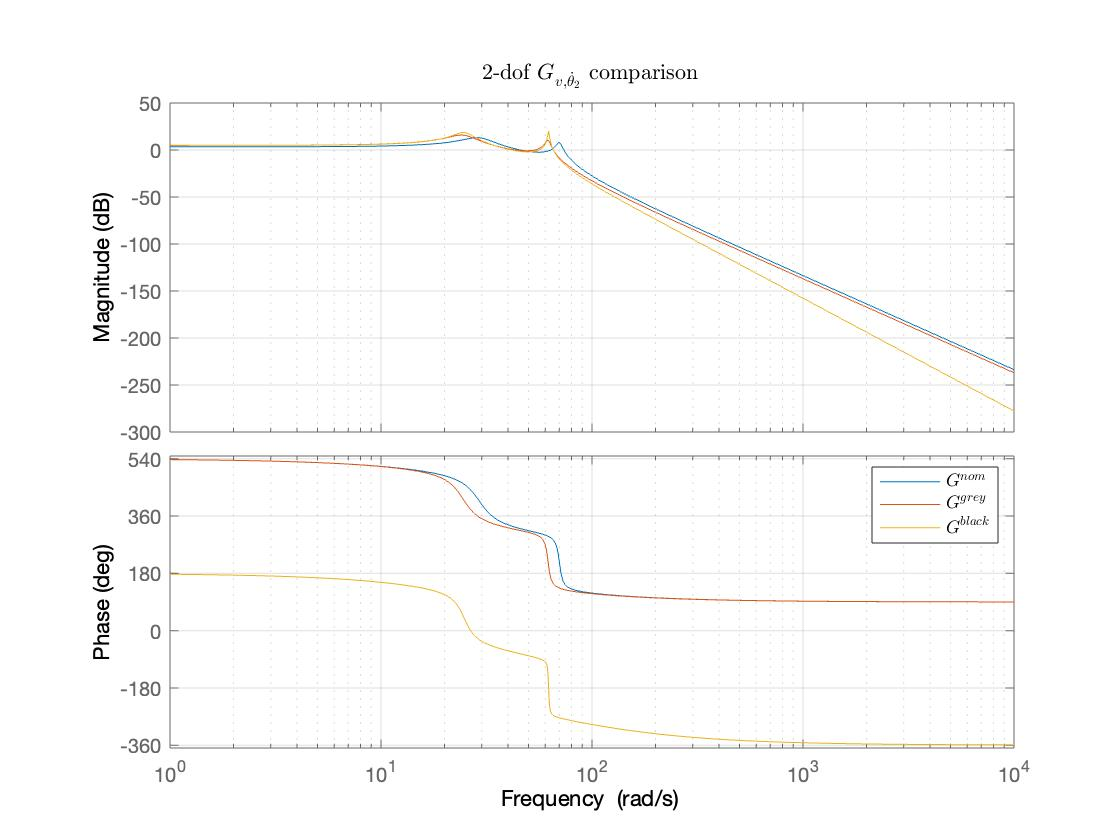
\includegraphics[width=\textwidth]{2dof_g_v_w2}
	\end{subfigure}
	\caption{2-dof system. Transfer functions comparison, no zeros in blackbox}
\end{figure*}

Following this approach, it has been observed that the resonance frequency of the identified model is lower that the nominal one, as the damping too.
Those differences can be immediately seen is the laboratory experiments: in particular, the ones with variable frequency sine wave. \\
It is important to remember that the speed measurement is noisy (the filter acts at very high frequency), because of the derivation from the encoder data. Hence, obtaining the position, by integrating the speed estimated by this model, would generate a drift that increases in time. \\


\section{Gray-box identification} \label{sec:gray_b_id}

\textit{Gray-box identification with a parametric error method of state-space time-domain} \\
\par The advantage of using a gray-box approach is that it maintains the mathematical model structure and tunes parameters based on experimental data. The starting model is defined on the nominal parameters (as illustrated in Paragraph "Mathematical description"), whose uncertainties are a-prior specified: in this way, the identification can change parameters in a well defined and constrained range, preserving a physical meaning. Specifically, masses parameters (inertia~$J$, friction~$B$) uncertainty is fixed manually~(the datasheet gives experimentally determined values); all the other parameters have an uncertainty range specified according to the reference manuals.
% table: nominal and identified parameters, uncertainty of param
% ragionare se controproducente !!!!!

Operatively, data experiments have been collected and the estimation of the model has been performed by means of the function~\textit{greyest()}. The used measurements include the position of both motor and masses: this allows to have a larger and differentiated set of data.

Identification results are very satisfactory: the precision of the model with respect to the motor position data are between~$70 / 95\%$, while the masses positions precision is about~$75 / 99\%$. The lower values of precision are obtained with low speed experiments.

The identified model has a resonance frequency located in between the nominal and black-box ones, as expected. Moreover, data collected in laboratory are very close to the simulation performed by using this identified model, thus, all the controllers are based on this identification.
